\newpage
\section{Discussion}
\begin{wrapfigure}{l}{0.5\textwidth}     \centering       
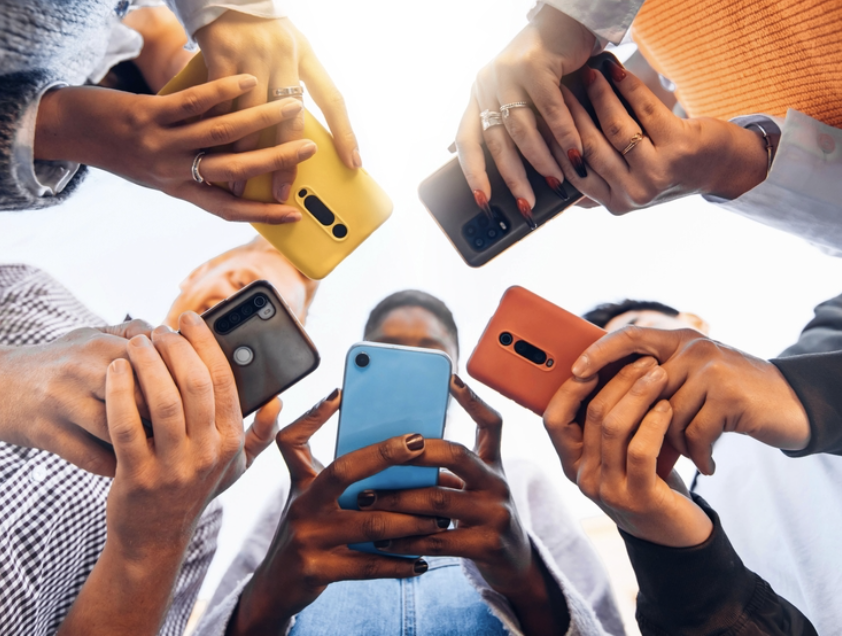
\includegraphics[width=0.4\textwidth]{phones.png}
\caption{\label{fig:latbrain}Teens have increasing access to phones (I will add a more relevant figure here for an actual FYP)}
\end{wrapfigure}

As hypothesized, passive social media use was associated with worse mental health than active social media use. As teens spend more time on social media, and the social connections that are of vital importance to adolescent development move online \citep{hollensteinreview2024}, it is important to understand how adolescents are spending their time in this digital world (see Figure~\ref{fig:latbrain}). The present study contributes to that understanding. Future research should consider using daily diary methods to better capture adolescent emotion and how those emotions are regulated by or simply relate to digital activities. Without understanding these relationships, we cannot understand adolescent development in the modern world.



